\documentclass{article}
\usepackage[T1]{fontenc}
\usepackage[utf8]{inputenc}
\usepackage{listings}
\usepackage{color}
\definecolor{red}{rgb}{0.6,0,0} % for strings
\definecolor{green}{rgb}{0.25,0.5,0.35} % comments
\definecolor{purple}{rgb}{0.5,0,0.35} % keywords
\definecolor{docblue}{rgb}{0.25,0.35,0.75} % javadoc
 
\lstset{
	basicstyle=\normalsize\ttfamily,
	keywordstyle=\color{purple}\bfseries,
	stringstyle=\color{red},
	commentstyle=\color{green},
	morecomment=[s][\color{docblue}]{/**}{*/},
	tabsize=4,
	showspaces=false,
	showstringspaces=false
}
	
\usepackage{graphicx}
\usepackage{fancyhdr}
\usepackage[margin=1.2in]{geometry}
\geometry{a4paper, left=20mm, right=20mm, top=20mm, bottom=20mm}
\linespread{1.5}
\begin{document}

\begin{titlepage}
	\begin{center}
		{\LARGE College of Engineering, Trivandrum}\\[3cm]
		\linespread{1.2}\huge {\bfseries Microprocessor Lab}\\[3cm]
		\linespread{1}
		
\includegraphics[width=8cm]{img/emblem.jpeg}\\[1cm]
		{\Large Gokul K\\ S6 CSE \\ Roll No: 21\\ TVE18CS021 }\\[1cm]
		\textit{ }\\[1cm]
		{\LARGE 
			Department of Computer Science\\[0.2cm]
			\today 
		}
	\end{center}
	
\end{titlepage}
\large

\newpage
\setlength{\headheight}{15.2pt}
\pagestyle{fancy}
\fancyhf{}
\fancyhead[RO]{\fontsize{12}{12}\selectfont\nouppercase\leftmark} 
\fancyhead[LO]{\fontsize{9}{12}\selectfont\nouppercase\rightmark} 

% Use the current experiment file from experiments/ folder
\section{Fibonacci Series}
\subsection{Aim}
To print the fibonacci series and the sum of its odd and even elements

\subsection{Code}
\begin{lstlisting}
DATA SEGMENT
  n DW 8 
  series DW 10 DUP(?)
  sumOdd DW 0
  sumEven DW 0
ENDS DATA   

CODE SEGMENT
ASSUME CS:CODE, DS:DATA
START:
  MOV AX, DATA
  MOV DS, AX
  MOV CX, 00
  MOV BX, 01
  LEA SI, series
  MOV [SI], 00
  ADD SI, 2
  
FIBLOOP:
  MOV AX, CX
  ADD AX, BX
  MOV BX, CX
  MOV CX, AX
  CMP CX, n 
  JG SUMLOOP
  MOV [SI], CX
  ADD SI, 2
  JMP FIBLOOP 
  
SUMLOOP:
  MOV AX, [SI]
  TEST AX, 01H
  JNZ ADDODD
  MOV AX, [SI]
  ADD sumEven, AX
  JMP INCR

ADDODD:
  MOV AX, [SI]
  ADD sumOdd, AX

INCR:
  SUB SI, 2
  CMP SI, series
  JLE EXIT
  JMP SUMLOOP

EXIT:
  MOV AH, 4CH
  INT 21h
ENDS CODE
END START
\end{lstlisting}

\subsection{Output}
\begin{center}
	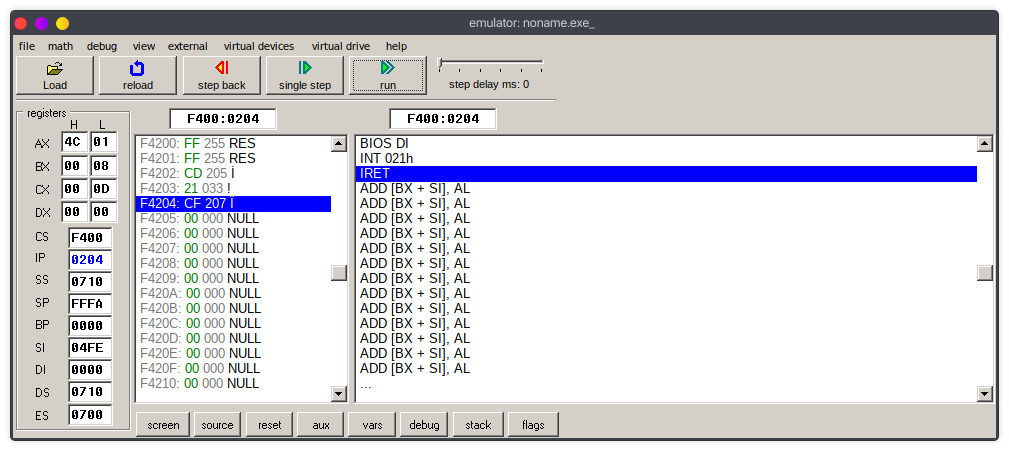
\includegraphics[width=0.90\textwidth]{img/pq1/ss1.png}\\
	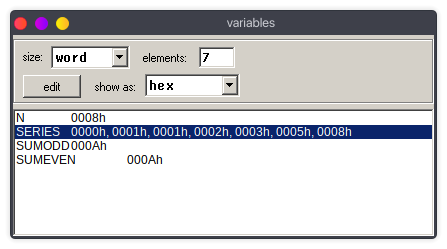
\includegraphics{img/pq1/ss2.png}
\end{center} 

\subsection{Result}
The program for printing fibonacci series was written and its output verified
\end{document}